% File acl2020.tex
%% Based on the style files for ACL 2020

\documentclass[11pt,a4paper]{article}
\usepackage[hyperref]{acl2020}
\usepackage{times}
\usepackage{latexsym}
\usepackage{amsfonts}
\usepackage{amsmath}
\usepackage{graphicx}

\renewcommand{\UrlFont}{\ttfamily\small}

% This is not strictly necessary, and may be commented out,
% but it will improve the layout of the manuscript,
% and will typically save some space.
\usepackage{microtype}

\aclfinalcopy % Uncomment this line for the final submission
%\def\aclpaperid{***} %  Enter the acl Paper ID here

%\setlength\titlebox{5cm}
% You can expand the titlebox if you need extra space
% to show all the authors. Please do not make the titlebox
% smaller than 5cm (the original size); we will check this
% in the camera-ready version and ask you to change it back.

\newcommand\BibTeX{B\textsc{ib}\TeX}

\title{Multi-Agent Reinforcement Learning in Zombie-Survival Games}

\author{
  Peter Hollows
  \thanks {
    Group submission for the final paper of XCS229ii,
    \mbox{Stanford Center for Professional Development}.
    Code available at https://github.com/captainpete/zombie-survival.
  }
  \\ \texttt{stanford@dojo7.com} \\
  \And
  Mark Presser
  \footnotemark[1]
  \\ \texttt{mark.presser95@gmail.com} \\
}

\date{}

\begin{document}
\maketitle
\begin{abstract}
  We investigate challenges of agent design using
  multi-agent zero-sum game called ``Zombie-Survival'' 
  in which we train 7 agents (2 survivors, 5 zombies)
  under different scenarios using the same reward function
  to investigate how different environmental dynamics
  can lead to very different learned policies.

  We show how state-space compression can improve the stability of a learned policy,
  how a health mechanism that impacts maximum speed can change the dominant strategy,
  and how arming the survivors with projectile weapons can lead to a social dilemma.

  Ultimately the survivors do not prevail.
\end{abstract}

\section{Introduction}

Reinforcement Learning (RL) methods have enjoyed recent popularity,
in part due to widely publicized successes on challenging tasks \citep{Silver1140,badia2020agent57,alphastarblog,barth2018distributed},
and the availability of quality open-source frameworks containing implementations of state-of-the-art models \citep{1606.01540,hoffman2020acme,stable-baselines}.

Though RL methods exceed human-level performance in some tasks such as
simulated games, network optimisation \citep{chen2018auto,mao2019learning,valadarsky2017learning} and even flying helicopters \citep{abbeel2006application},
there are many challenges discouraging the real-world deployment of RL systems \citep{dulacarnold2019challenges}.

\subsection{The Reality Gap}

One of these challenges is that most RL methods are not sample-effecicient, meaning the policy learner needs a lot of data before an effective policy can be found.
Often, there is not enough data available, or it cannot be captured safely (consider an autonomous driver learning the best policy for a near-crash scenario, where it will make mistakes in order to learn).
To work around these issues, RL policies intended for real-world control tasks are usually trained in simulated environments before being further trained or deployed in the real-world.

However, simulations often do not capture all the relevant real-world dynamics, so it can be difficult to transition a policy from the simulator to reality.
This difficulty, known as the ``reality gap'', is often mitigated by adding noise \citep{jakobi1995noise} to the simulation (to mimic noisy sensors and stochastic dynamics),
or by sufficiently improving the simulation to model the relevant dynamics.

\subsection{Multi-Agent RL}

When designing an RL agent for use in cooperative settings like factories, or competitive setting like markets,
we have to allow for the fact that other agents may be present in the environment and may change their behavior in response to the activity of other agents.
Training multiple agents concurrently in simulation can capture some of the dynamics around agents learning to respond to each other's actions.
However, there are technical challenges to do with non-stationarity that prevent success in the naive approach of using multiple, single-agent algorithms.

These technical issues motivated the Multi-Agent Deep Deterministic Policy Gradient (MADDPG) algorithm \citep{lowe2020multiagent}.
MADDPG addresses some issues in multi-agent learning, and allows running experiments that explore the emergence of competitive and cooperative policies in complex environments.

\subsection{Overview}

We explore the impacts of environmental dynamics on policy evolution 
in the multi-agent RL setting.
We use MADDPG to train multiple agents in a mixed competitive-cooperative simulated environment called ``Zombie-Survival''.
We make several modifications to the environment in order to observe agent behavior under different scenarios.

In (\ref{sec:background}) we review theory, training algorithms, and aspects of agent design.
In (\ref{sec:game}) we detail the basic simulation environment.
In (\ref{sec:baseline}) we detail the experimental setup and initial results.
In (\ref{sec:anon}) we investigate partial observability, and how compression of the observation-space can speed policy discovery.
In (\ref{sec:health}) we alter the environment to cause a change in the value-function (keeping reward unchanged) to study the impact on learned policies.
In (\ref{sec:arms}) we arm the survivors with projectile weapons to investigate how this additional capability can make it harder for agents to achieve their objectives.
We present methods and results for each scenario, and conclude with a discussion of our findings (\ref{sec:discussion}).

\section{Background}
\label{sec:background}

\subsection{The Markov Decision Process}

A Markov Decision Process (MDP) formalizes the interaction of an agent with an environment \citep{SuttonBarto}.
At every time step, an \emph{agent} receives observations of the \emph{state} of the \emph{environment}, and sends \emph{actions} to the environment.
The environment transitions from one state to the next over time, and actions from the agent can influence which states the environment transitions to.
At every time step, the agent receives a \emph{reward} based on the state of the environment.
In the case when state transitions are not independent (i.e. the chance of arriving in a state depends on visiting previous states), an agent's actions in a state can impact future expected rewards as well as immediate rewards.

RL algorithms attempt to solve the MDP in order to maximize return (reward over time).
This is done by learning a policy (a function that maps from state to action).
A policy can often be learned directly, or by learning a value function (a mapping from states and actions to expected returns) from which a policy can be extracted.

\subsection{Algorithms}

\paragraph{DQN} Q-Learning \citep{watkins} is an RL method that makes use of an action-value function $Q^\pi(s, a)$ corresponding to a policy $\pi$ (where $s$ is the state, and $a$ the action).
Deep Q-Learning Networks (DQN) \citep{2015Natur.518..529M} learn the action-value function $Q^*$ corresponding to the optimal policy by minimizing the loss function
\begin{equation}
  \mathcal{L}(\theta)=\mathbb{E}_{s,a,r,s'}[(Q^*(s,a|\theta)-y)^2],
\end{equation}
where $y=r+\gamma\max_{a'}\bar{Q}^*(s',a')$,
by repeatedly adjusting the parameters $\theta$ of the target action-value function $\bar{Q}$.
The Q-function can be expressed as $Q^{\pi}(s,a)=\mathbb{E}[R|s,a]$, where $R_t$ is the discounted sum of future rewards at time $t$, given by: $R_t=\sum_{k=t}^\infty\gamma(k-t)r_k$.
To reduce the variance of estimates for the above expectation, DQN makes use of an Experience Replay (ER) buffer that stores the experiences of many state transitions.

\paragraph{Policy-gradient} Policy-gradient (PG) methods learn a policy $\pi_\theta$, parameterized by $\theta$,
by sampling the gradient of a performance measure $J(\theta)$ with respect to $\theta$.

\begin{equation}
  \nabla_\theta J(\theta)=\mathbb{E}_\pi\left[Q^\pi(s, a) \frac{\nabla_\theta\pi_\theta(a|s)}{\pi_\theta(a|s)}\right]
\end{equation}

Learning a policy directly is useful in situations where extraction of a policy from a value function would be difficult (consider the scenario of a very large, or continuous action space).

REINFORCE \citep{Williams92simplestatistical} is a simple Monte-Carlo policy-gradient algorithm that uses all the steps in an episode to sample $Q^\pi(s,a)=\mathbb{E}_\pi[G|s,a]$ (where $G$ is the expected return of an episode) to make a policy update.
Because reward functions sometimes give high values for some states, this method can give high-variance gradient estimates.
This can be remedied by using a baseline $b(s)$ \citep{SuttonBarto}:

\begin{equation}
  \nabla_\theta J(\theta)=\mathbb{E}_\pi\left[(G-b(s)) \frac{\nabla_\theta\pi_\theta(a|s)}{\pi_\theta(a|s)}\right]
\end{equation}

\paragraph{Actor-critic} The Actor-Critic algorithm \citep{bhatnagar2009natural} improves on REINFORCE by learning a state-value function with baseline (critic), and an action-value function (actor) concurrently.
Actor-Critic also has the advantage that the parameters for both functions are updated at every step in an episode.
The policy gradient at each time step $t$ can be expressed:

\begin{equation}
  \nabla_\theta J(\theta)=\mathbb{E}_\pi\left[\delta_t \frac{\nabla_\theta\pi_\theta(a|s)}{\pi_\theta(a|s)}\right]
\end{equation}
\begin{equation}
  \delta_t = r_{t+1}+\gamma \hat{v}(s_{t+1}, w)-\hat{v}(s_t,w)
\end{equation}

where $\gamma$ is a discount parameter, and $\hat{v}(w)$ the state-value function with parameters $w$.

\paragraph{DPG} The Deterministic Policy Gradient (DPG) algorithm \citep{pmlr-v32-silver14} extend policy-gradient methods to deterministic policies.
A deterministic policy ($\mu_\theta$) maps a state to an action,
whereas a stochastic policy ($\pi_\theta$) provides a conditional probability of an action in a given state.

\begin{equation}
  \nabla_\theta J(\theta)=\mathbb{E}_s\left[\nabla_\theta \mu_\theta(a|s) \nabla_a Q^\mu(s,a)|_{a=\mu_\theta(s)}\right]
\end{equation}

DPG methods are suited to continuous control tasks
(taking the gradient of $Q^\mu$ with respect to $a$ requires the action space to be continuous).

\paragraph{DDPG} The Deep Deterministric Policy-Gradient algorithm \citep{lillicrap2019continuous} combines ideas from DPG and DQN.
In DDPG the actor and critic are approximated with neural networks.
DDPG uses target networks for both actor and critic, and makes use of an experience replay buffer to store agent trajectories.

\subsection{MADDPG}

Under MDP additional agents are regarded as part of the environment.
From the perspective of an agent, the influence on rewards from other agents can make it harder to learn a policy;
this is especially so when the environment contains other agents that are also learning policies,
because the other agents can cause the environment's dynamics to change while the agent is trying to learn them.

\citealp{lowe2020multiagent} showed that the chance of sampling a policy-gradient update for an agent in the direction of higher expected return decreases exponentially with the number of agents being trained in the shared environemnt.

MADDPG addresses this stabilitiy issue by using centralized critics.
In MADDPG, the critic $Q^\pi_i(x, a_1, a_2, ..., a_N)$ for agent $i$ has access to the actions of all $N$ agents, and some state information $x$.
%The critic is often only used in training, so it's possible to deploy MADDPG actors in continuous control tasks where knowledge of other actors' actions are not available.

Under MADDPG, agents agents are permitted to have different state and action spaces, and to be goverened by different reward functions.
We use the MADDPG algorithm for all agents within our scenarios.

% \subsection{Agent Design}
% 
% When implementing an RL system there are many important design decisions, some key considerations are:
% 
% \begin{itemize}
%   \item \emph{Algorithm}: Different algorithms are suited to different tasks. A selected algorithm will need to perform well with the selected action-space, state-space, reward function and environmental dynamics.
%   \item \emph{State-space}: The state-space describes how environmental observations are presented to the algorithm. Constructing the correct, relevant abstractions allow an agent to better learn the environment.
%   \item \emph{Action-space}: The action-space describes actions available to the agent. The level of abstraction here should be fine enough for precise control, but general enough for a policy to be easily learnable.
%   \item \emph{Reward function}: The reward function provides a scalar feedback value (positive or negative) to the agent. Some algorithms can model uncertainty in the reward function \citep{ghavamzadeh2016bayesian}, but most expect a point-estimate rather than a distribution. Crafting a consistent reward function that reflects the exact desires of the designer can be challenging \citep{leike2017ai}. Some algorithms can infer the a reward function from feedback \citep{ng2000algorithms}, but most simply try to maximize the explicit reward given by the function.
% \end{itemize}
% 
% In our scenarios we implement a simple reward function that creates a zero-sum game, where one agent's loss is another's gain.
% Our investigation examines the effect of design choices relating to the state-space and action-space, and how those impact the emergence of policies.

\section{Scenarios}
\label{sec:scenarios}

\subsection{Zombie-Survival Game}
\label{sec:game}

The Zombie-Survival scenarios cover a set of games simulating survivors and zombies in a zombie-apocalypse scenario.
When a zombie is in physical contact with a survivor this results in a `bite' between zombie and survivor.
Zombies attempt to bite survivors and are rewarded for each step they are in contact.
Survivors attempt to distance themselves from zombies and are penalized every time they are bitten.
Survivors can suffer a bite from multiple zombies in the same time step.

Zombies have the advantage of numbers, whereas survivors have the advantage of faster accleration and a higher maximum speed (Table \ref{game-settings}).

\begin{table}
\centering
\begin{tabular}{lrr}
\hline \textbf{Setting} & \textbf{Survivors} & \textbf{Zombies} \\ \hline
  world size ($m$) & 2x2 & 2x2 \\
  timestep ($s$) & 0.1 & 0.1 \\
  episode length ($s$) & 10 & 10 \\
  num. agents & 2 & \textbf{5} \\
  agent radius ($m$) & 0.05 & 0.05 \\
  agent mass ($kg$) & 1.0 & 1.0 \\
  acceleration ($ms^-2$) & \textbf{4.0} & 3.0 \\
  max. speed ($ms^-1$) & \textbf{1.3} & 1.0 \\
  bite reward & -10 & +10 \\
\hline
\end{tabular}
\caption{\label{game-settings} Scenario settings. }
\end{table}

\subsection{Scenario: Baseline}
\label{sec:baseline}

We modify the ``Predator-prey'' particle environment from \citealp{lowe2020multiagent}, which implements a multi-agent environment with a continuous action-space, a fully-observable state-space, and basic 2D physics.
Each agent is represented as a circle that has mass, position, velocity, velocity dampening, maximum acceleration, and maximum speed.
The predator-prey environment uses reward shaping to discourage agents from moving out of bounds; we remove this additional term in the reward function and implement fixed boundary walls.
We implement the biting rules, modify the agent count and adjust the agents' physical capabilities (Table \ref{game-settings}).
We run multiple experiments in which we train agents over 10,000 episodes.

\subsection{Results: Baseline}

\begin{figure}
  \centering
  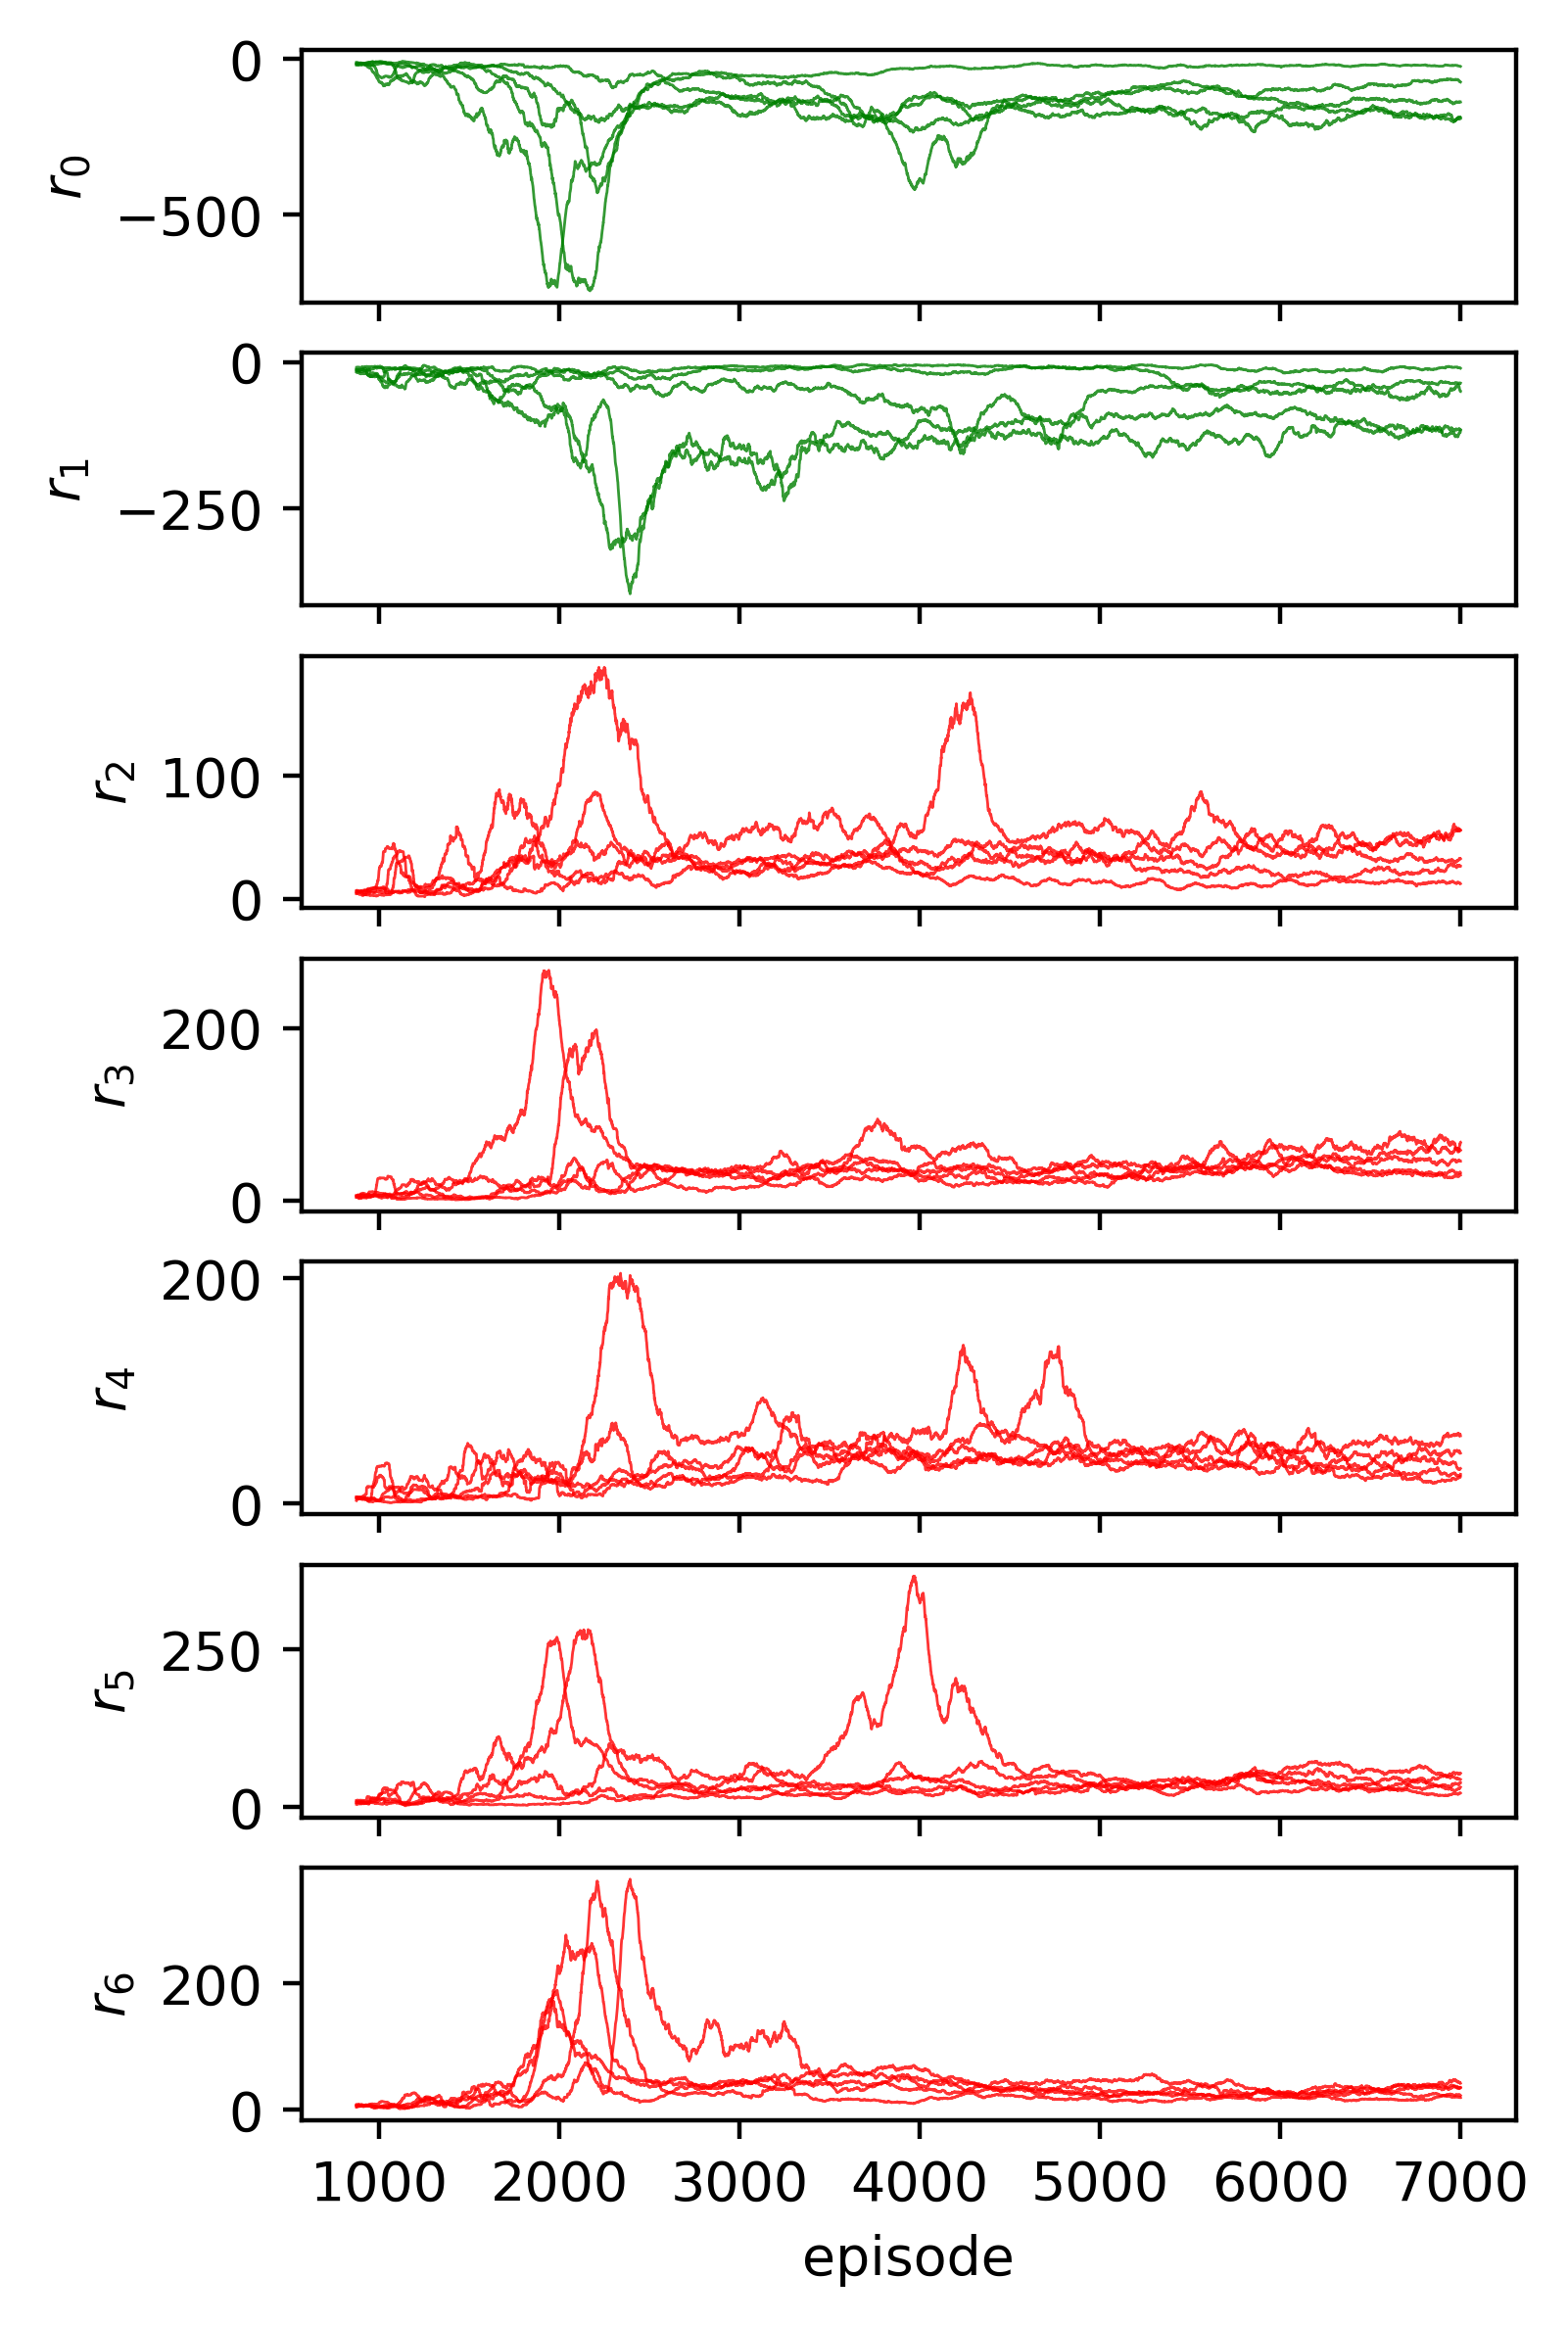
\includegraphics[width=0.5\textwidth]{figures/baseline_reward.png}
  \caption{
    Reward (moving average over 100 episodes) for survivors (green) and zombies (red) for 10 training runs.
    Agents experience policy shifts between episode 2000 to 6000.
    Policies stabilize after 7000 episodes.
  }
  \label{fig:baseline_reward}
\end{figure}

\paragraph{Variability} We observed variability in policy convergence between training runs.
Figure \ref{fig:baseline_reward} shows agent reward graphs over multiple runs.
The reward trace for $r_5$ shows the zombie agent experienced a spike in reward corresponding to a drop in reward for a survivor in $r_0$
that occurred only once in 10 training runs.
Most agents show a similar pattern for at least one run.

\begin{figure}
  \centering
  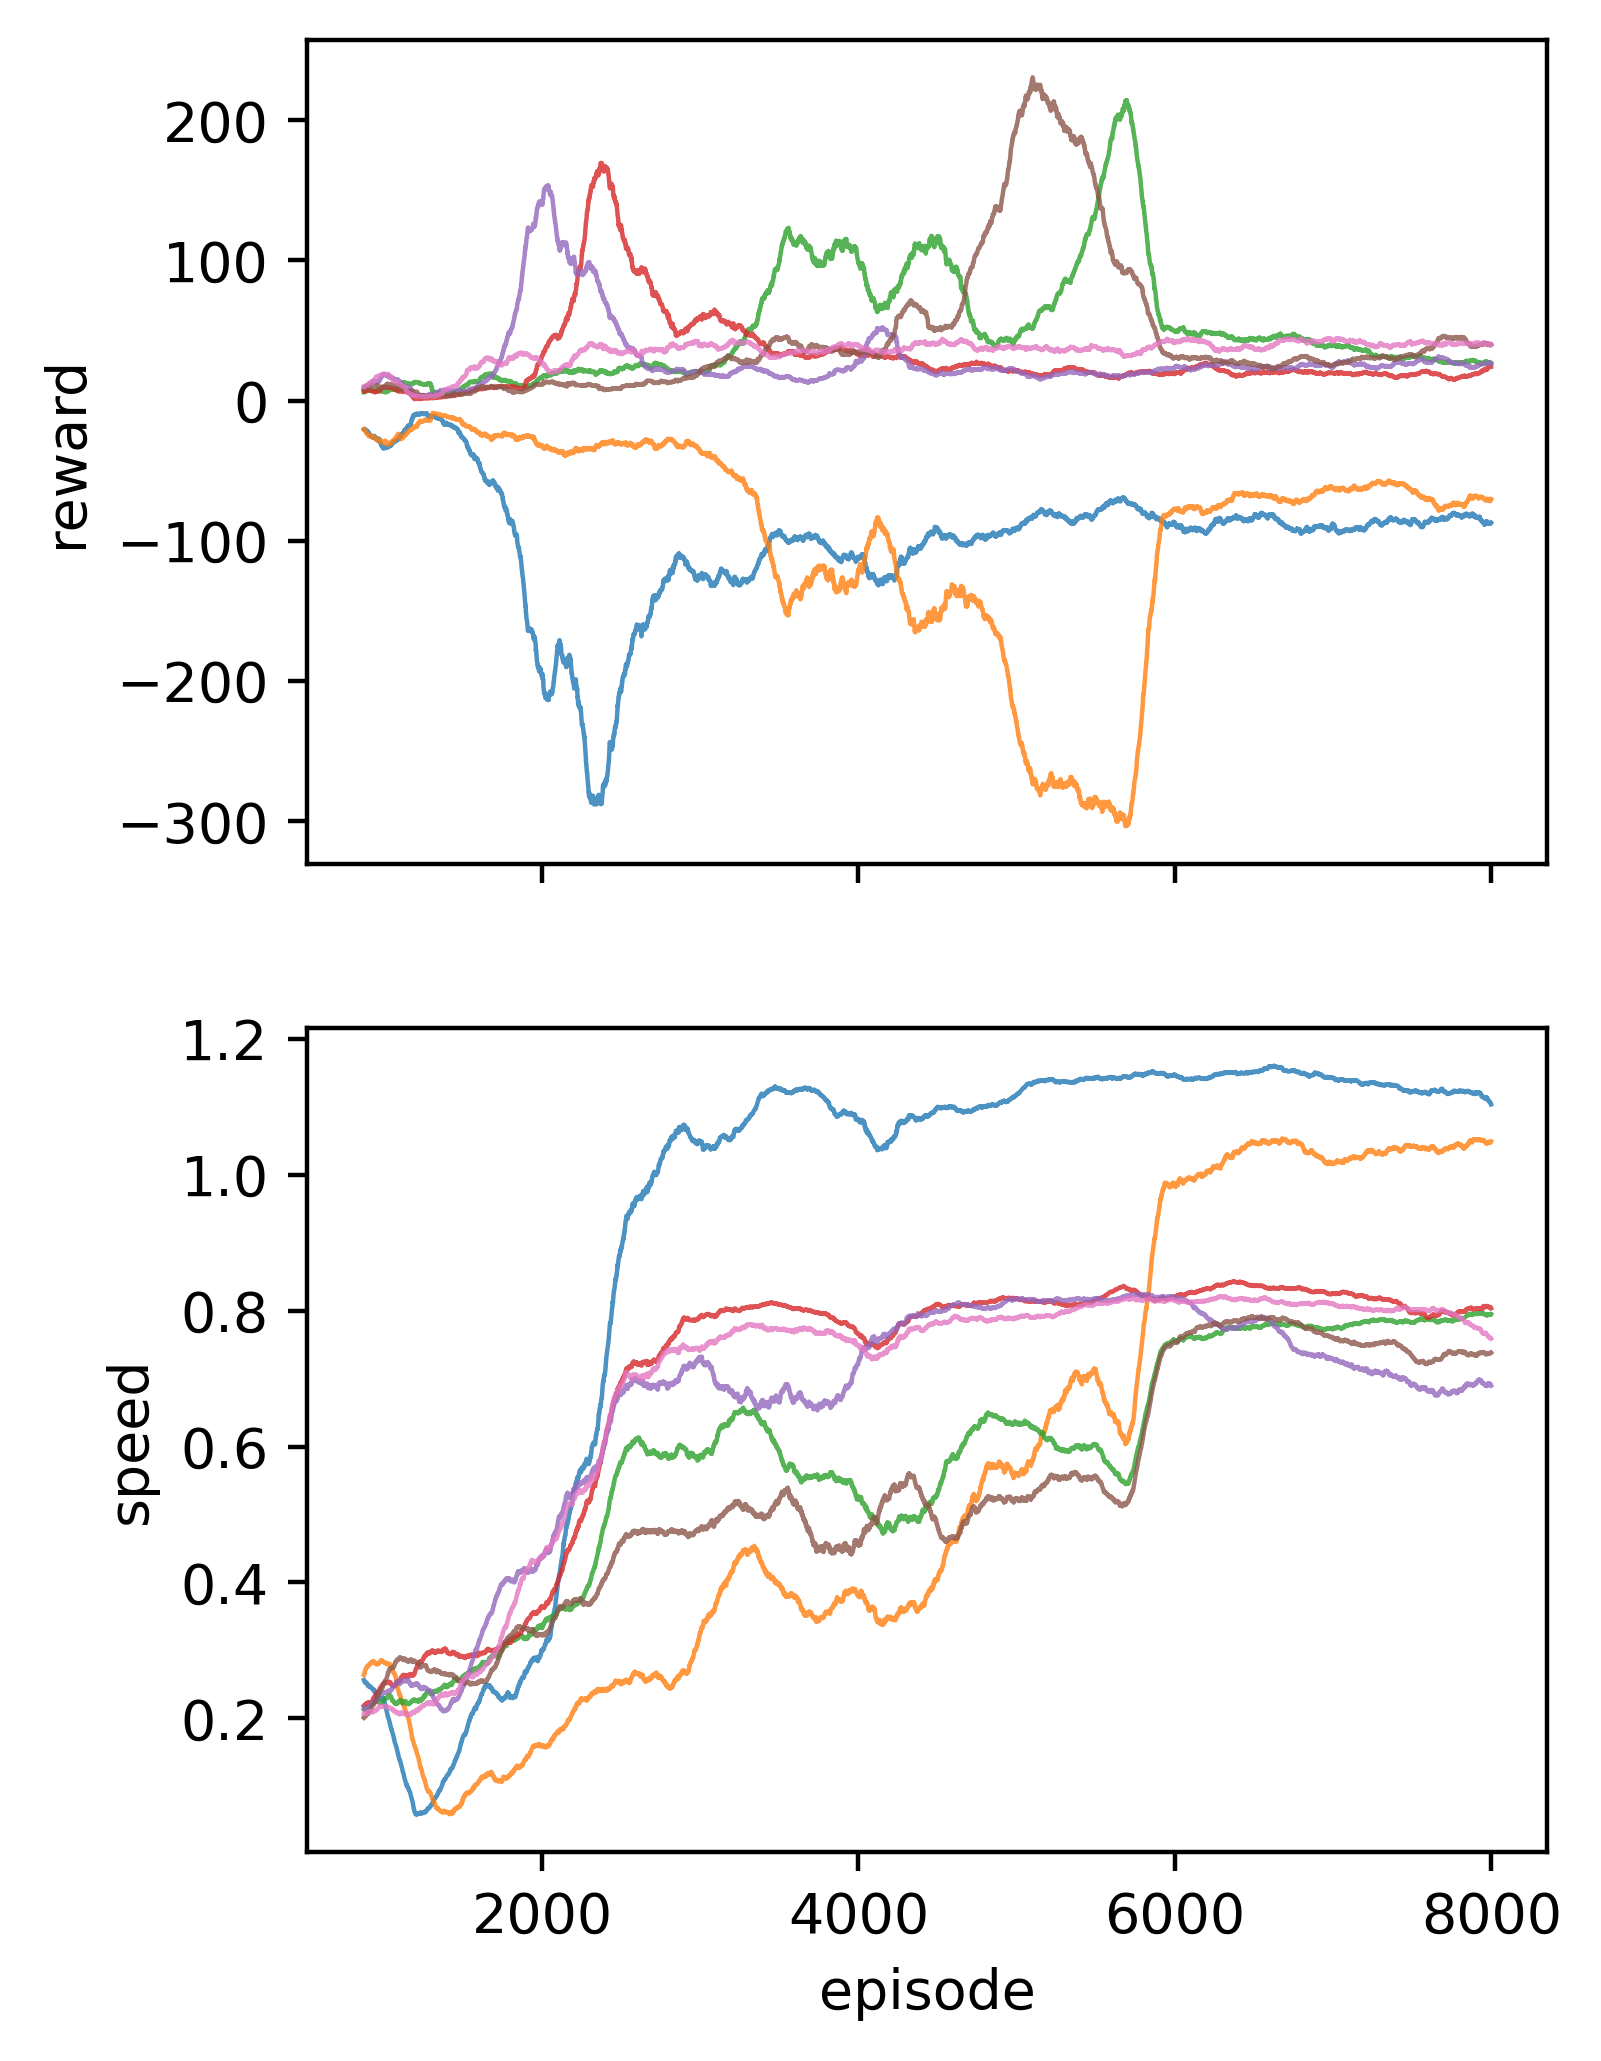
\includegraphics[width=0.5\textwidth]{figures/baseline_speed.png}
  \caption{
    Reward and average speed (moving averages over 200 episodes)
    for all agents in a single training run of the \emph{baseline} scenario.
    Survivors (blue and orange) learn faster movement at different times.
  }
  \label{fig:baseline_speed}
\end{figure}

\paragraph{Target fixation} On further investigation we discovered the reason for the variability; a zombie usually fixates on a target, but zombies learn policies at different rates.
Figure \ref{fig:baseline_speed} shows speed and reward over time for a single training run.
We see that one survivor is not pursued as often to start with, but then recieves increasing attention from zombies learning to persure it.
Following this attention the survivor learns to move much faster.
We observed similar patterns in other runs.

In the \emph{baseline} state-space, every agent is unique, so all agents have to learn the expected reward specific to every other agent.
We propose that from an agent's perspective, when considering reward the most important thing about another agent is whether they are a survivor or a zombie, not necessarily which survivor or zombie.
We'd prefer agents learn general policies that consider other agents as exchangeable within a team.

\subsection{Scenario: Anonymity}
\label{sec:anon}

In the \emph{anonymity} scenario we modify the \emph{baseline} scenario to introduce partial observability.
We re-order agents' state vectors each step so that agents within teams are ordered by distance to the observing agent.
To a survivor, a zombie now appears the same as any other zombie, and does not have identity by virtue of index in the state vector.
This reduces the size of the state-space considerably, and allows agents to learn policies that focus on nearby agents.

We expect both survivors and zombies to learn more general policies with faster convergence than in the \emph{baseline} scenario.
We also expect to see zombies chasing which ever survivor is easiest to chase, rather than fixating on a single survivor.

\subsection{Results: Anonymity}

We observed less variance in convergence to a stable policy (as judged by average speed and reward) when compared to \emph{baseline} (see Figure \ref{fig:anon_base_compare}).
We also observed more uniform persuit and biting (see Figure \ref{fig:anon_base_dist_bite}).

\begin{figure}
  \centering
  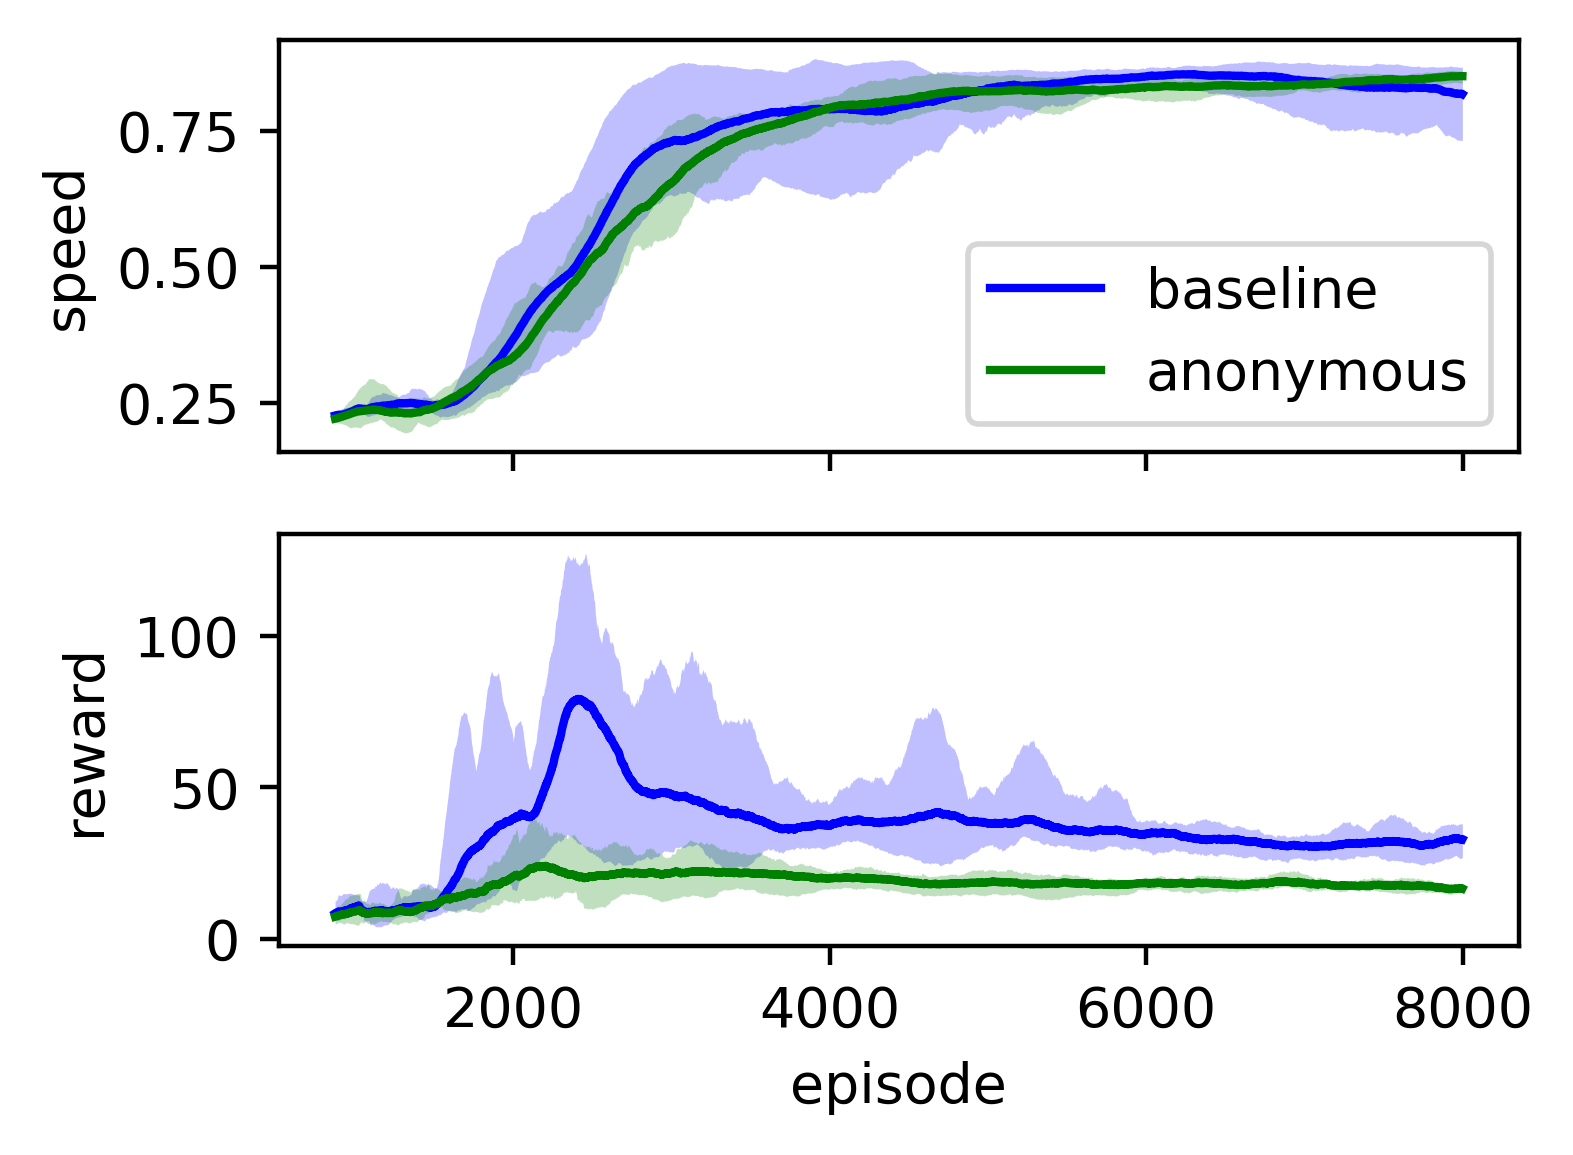
\includegraphics[width=0.5\textwidth]{figures/anon_base_compare.png}
  \caption{
    Speed and reward evolution for baseline and anonymous scenarios over 8 training runs.
    Results taken as moving averages over 200 episodes prior to aggregation.
  }
  \label{fig:anon_base_compare}
\end{figure}

\begin{figure}
  \centering
  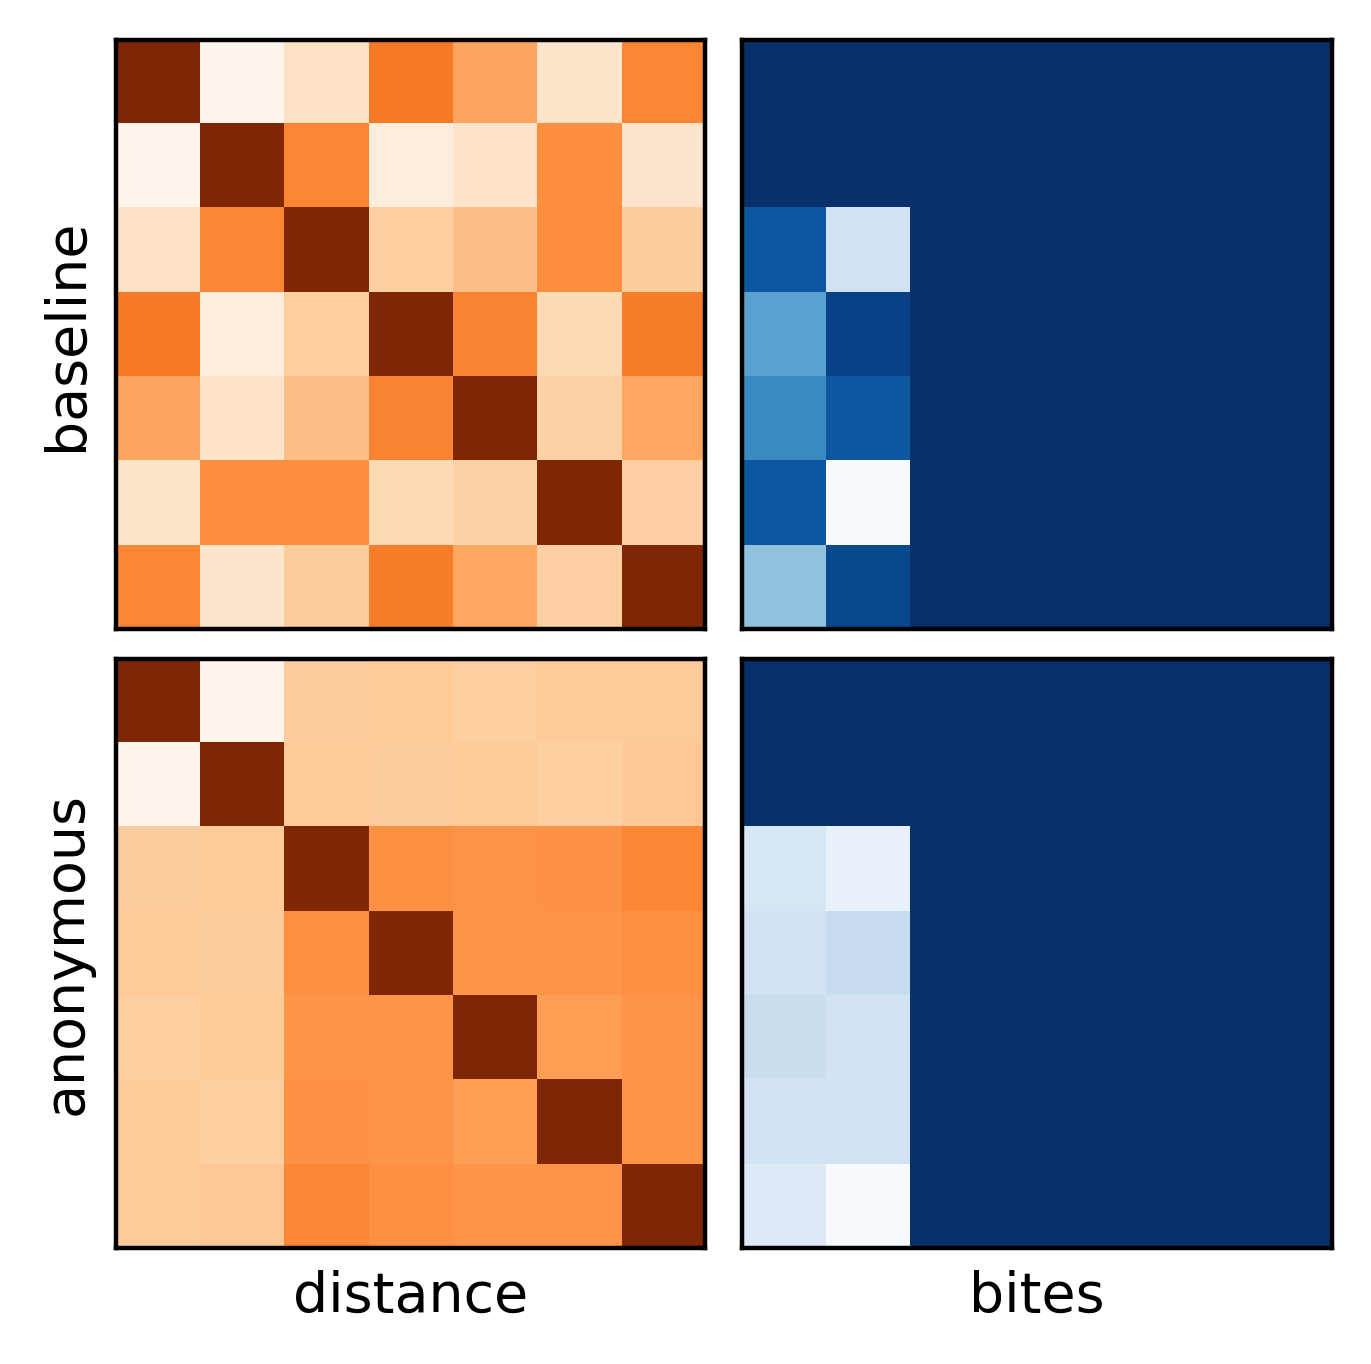
\includegraphics[width=0.5\textwidth]{figures/anon_base_dist_bite.png}
  \caption{
    Distance and bite count comparison between \emph{baseline} and \emph{anonymous} scenarios.
    Plot colors indicate average distance and average bite count per episode, averaged across the last 5000 episodes of a single training run.
    Both axes are agent indexes, and shade of color indicates relative value with white being the highest value.
  }
  \label{fig:anon_base_dist_bite}
\end{figure}

\subsection{Scenario: Health}
\label{sec:health}

In the \emph{health} scenario we modify the \emph{anonymity} scenario to introduce a health mechanism for survivors.
Survivors start each episode with 100\% health, which for survivors is discounted ($\gamma=0.99$) every bite (one bite per zombie in contact per time step).
An agent's health level is added to the private observation space for the agent.
Maximum speed at each step is limited to the fraction of health remaining.
If a survivor is bitten too often, they become slower than the zombies and risk being overrun, leading to a large amount of bites for the remainder of the episode.

This scenario does not alter the reward function, but increases the variance and magnitude of state-value estimates for both zombies and survivors.
Additionally, this scenario shifts the balance of power heavily toward the zombies.
We expect to see survivor policies emerge that are more risk-averse, and to see zombies elect to chase slower-moving survivors.

\subsection{Results: Health}

\paragraph{Breakout} Compared to the \emph{anonymous} scenario, agents in the \emph{health} scenario were slower on average (see Figure \ref{fig:anon_health_compare}, plot 1).
This slowdown occurred before the reward ramp-up caused by zombies learning to immobilize survivors.
In part the initial slower speeds can be explained through partial health reductions, but rendering the simulation frames provided another explanation.
In previous scenarios, survivors would run into walls at maximum speed to bounce back through the persuring group of zombies without losing speed.
The bouncing strategy sacrifices reward but allows a survivor to keep their distance ahead of the pursuing zombies after the manouver.
In the \emph{health} scenario, this strategy becomes unsustainable, as every contact with a zombie reduces the survivors maximum speed leading to a very bad outcome after only a few bounces.

\paragraph{Game-over} We measured a drastic increase in average zombie reward (Figure \ref{fig:anon_health_compare}, plot 2) due to zombies learning to immobilize and bite survivors.
In most cases, one survivor would succumb to the zombies first.
Zombies learn that moving in the direction of the slower-moving survivor leads to states with higher expected value, so they collaborate in slowing down one survivor, leaving the other survivor to escape out of harm's way (Figure \ref{fig:anon_health_compare}, plot 4).

\paragraph{Survivor competition} Survivors that were not the focus of `zombie collaboration' learned to stay out of the way by distancing themselves from the other survivor and their zombie entourage (see Figure \ref{fig:health_survivor_dist}).

In some episodes, survivors would trade places as the focus of zombie attention.
A fast moving survivor with zombies in persuit would move directly toward the other survivor (who was often be keeping their distance in a corner).
The first survivor would have higher velocity, and use it to risk a wall-bounce manouver near the second slower-moving one.
The first survivor in this instance would retain the speed required to escape while the zombies switched their persuit to overrun the second survivor.
We found it difficult initially to predict which survivor would ultimately attract the zombies, but around episode 6000 the survivors started to better avoid this trap by moving away from areas that would soon receive zombies.

\begin{figure}
  \centering
  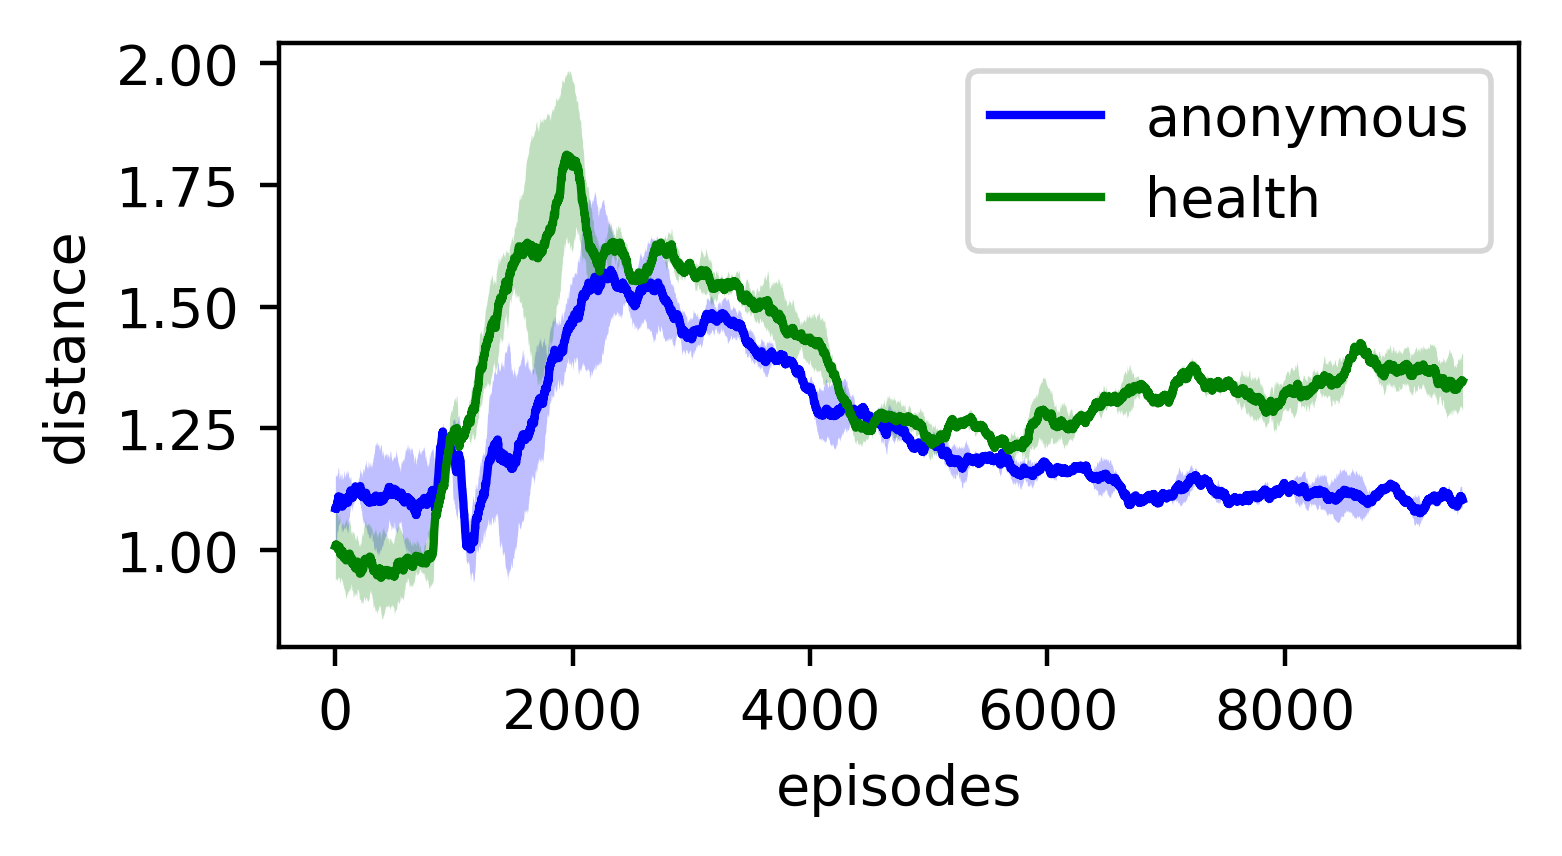
\includegraphics[width=0.5\textwidth]{figures/health_survivor_dist.png}
  \caption{
    Distance between survivors in the \emph{health} scenario.
    Survivors learn to keep their distance from one another more than in the \emph{anonymous} scenario.
    Results taken as moving averages over 200 episodes prior to aggregation.
  }
  \label{fig:health_survivor_dist}
\end{figure}

The introduction of the health dynamic moved the simulation closer to what we consider a `more realistic' zombie-survivor scenario.
The change in state-space and environmental dynamics lead to a very different movement policy for agents without changing the reward function.

\begin{figure}
  \centering
  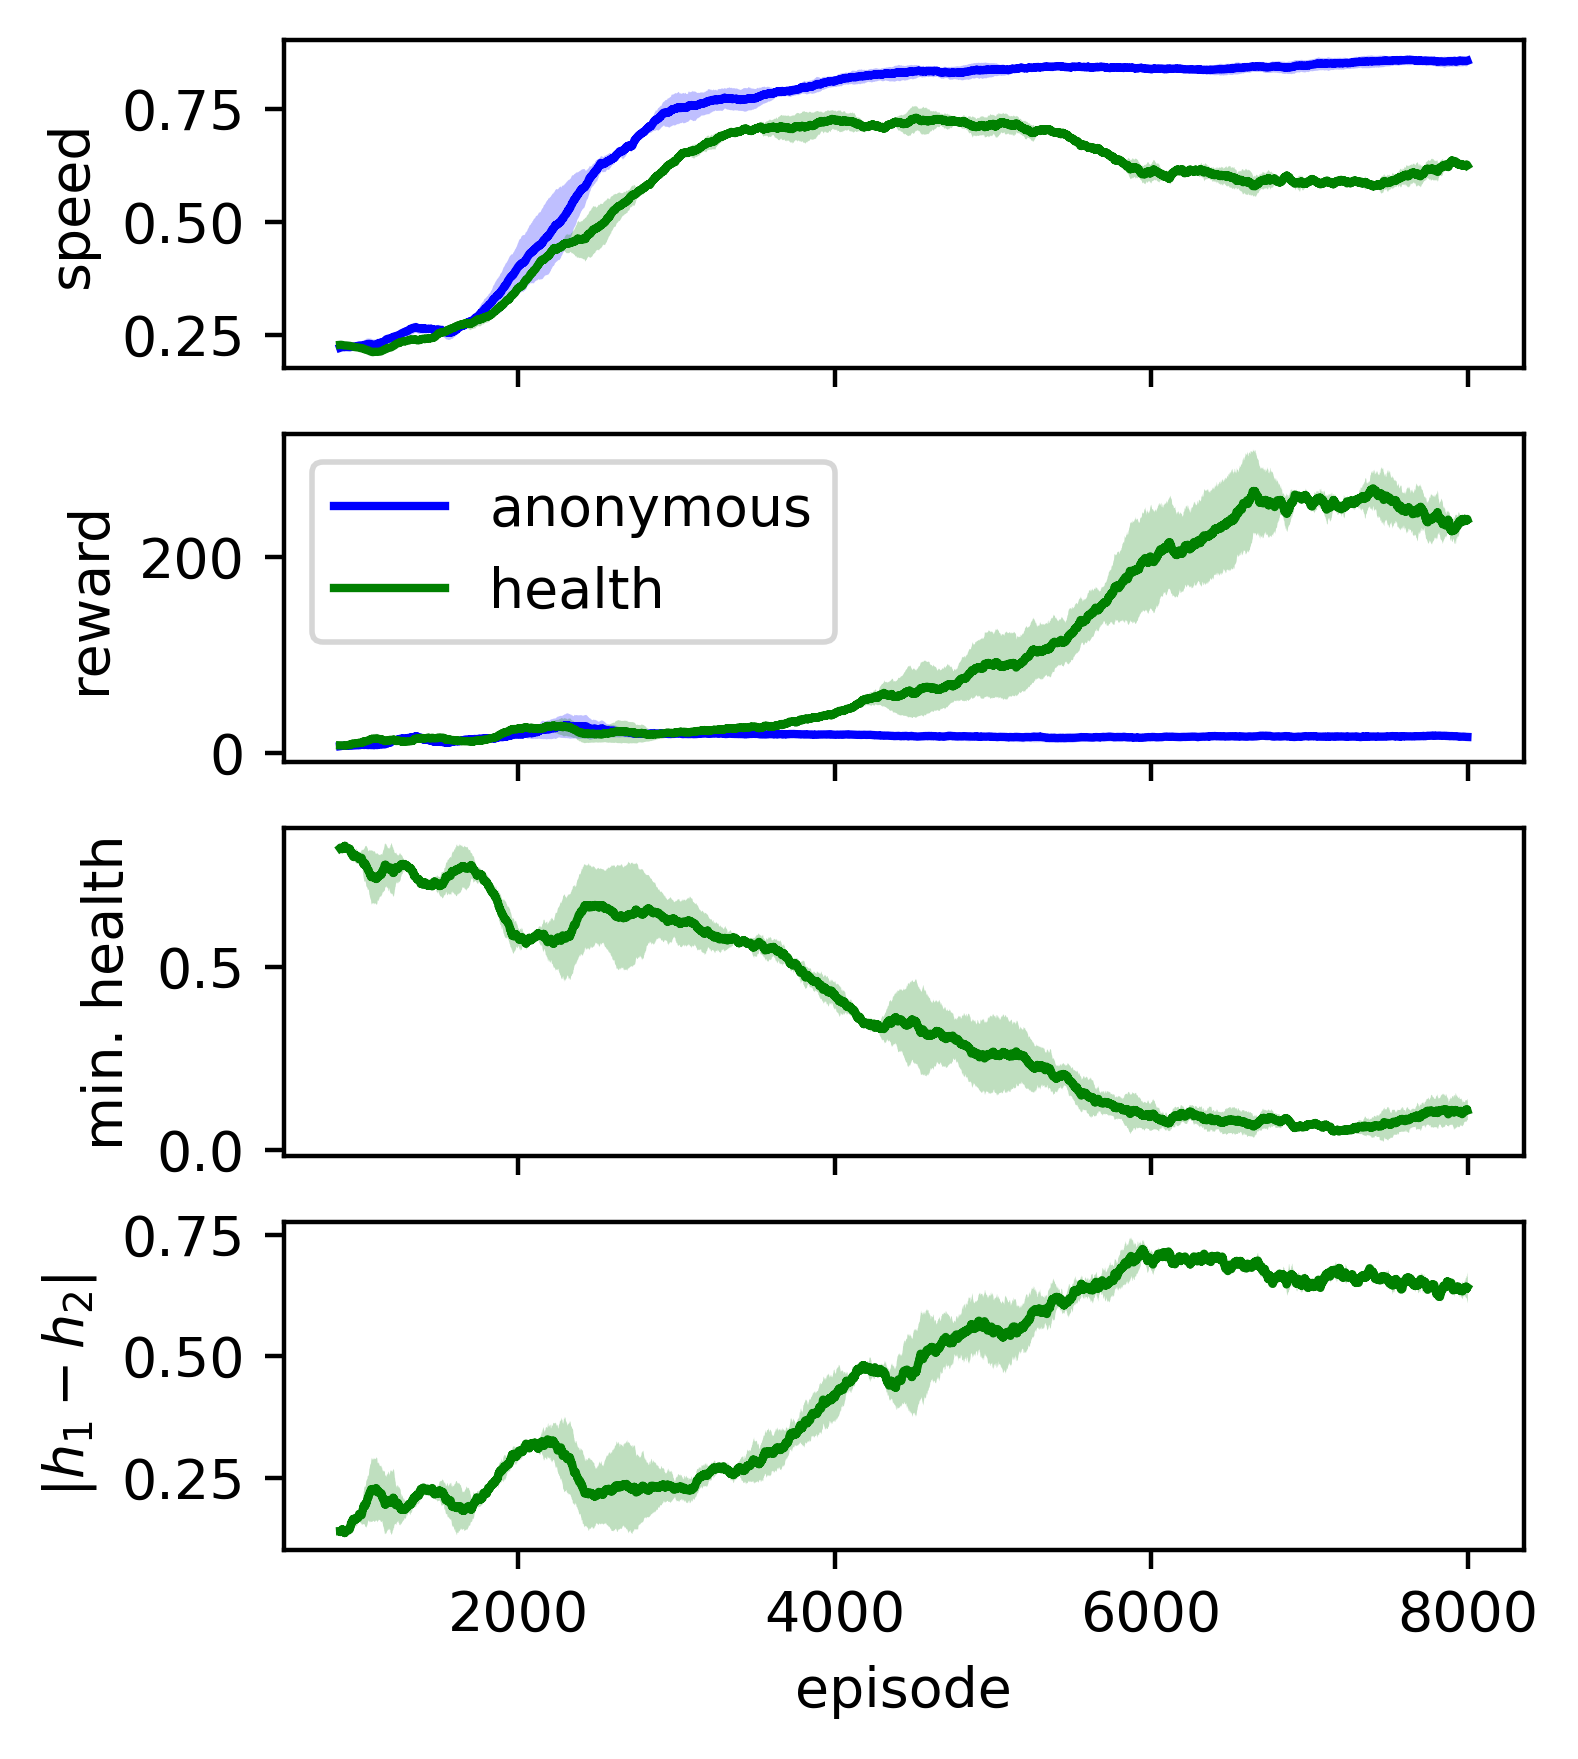
\includegraphics[width=0.5\textwidth]{figures/anon_health_compare.png}
  \caption{
    Comparison between \emph{anonymous} and \emph{health} scenario policy evolution.
    Results taken as moving averages over 200 episodes prior to aggregation.
    Plot 1: average speed of all agents.
    Plot 2: average reward of zombies.
    Plot 3: lowest health of all survivors at the conclusion of an episode.
    Plot 4: the difference between survivor health at the conclusion of an episode.
  }
  \label{fig:anon_health_compare}
\end{figure}

\subsection{Scenario: Armed}
\label{sec:arms}

In the \emph{armed} scenario we attempt to rebalance the game by modifying the \emph{health} scenario to arm the survivors with firearms.
Each armed agent has a firearm that fires 2 shots simultaneously when activated.
On firing, two rays are cast with a small random spread ($\angle ray \sim \mathcal{N}(\angle aim, 2^\circ)$).
When a ray first intersects with another agent it is counted as a `hit'.
An agent experiencing a hit has their health level reduced (by 0.2).
Armed agents require time to reload (1 step).
Both zombies and survivors can be rendered immobile through reduced health by being hit too often.

We add a normalized current heading and relative heading of locations of other agents to a each survivor's state-space, as well as a normalized time remaining until the firearm is reloaded.
Zombies and the other survivor do not observe a survivor's aim or reloading states.

Reloading is automatic and does not require an action.
The continuous aiming action (left and right) modifies angular velocity of aim directly (rather than through acceleration) up to a maximum speed of 1 revolution per second.
The firing mechanic is implemented as a `trigger pressure' which determines the probability of a loaded firearm discharging in a given timestep.
Firing probability is implemented as the sigmoid function $p(fire) = \frac{health}{1+e^{20(x-0.5)}}$, where $x$ is pressure on the trigger (note the ability for a survivor to fire depends on their health).

We expect introducing the arms mechanic will move the balance of power back toward the survivors.
We're not sure if the social dilemma presented will cause the survivors to fire on one another more often than the zombies,
but make no adjustment to the reward function to discourage it.

\subsection{Results: Armed}

\begin{figure}
  \centering
  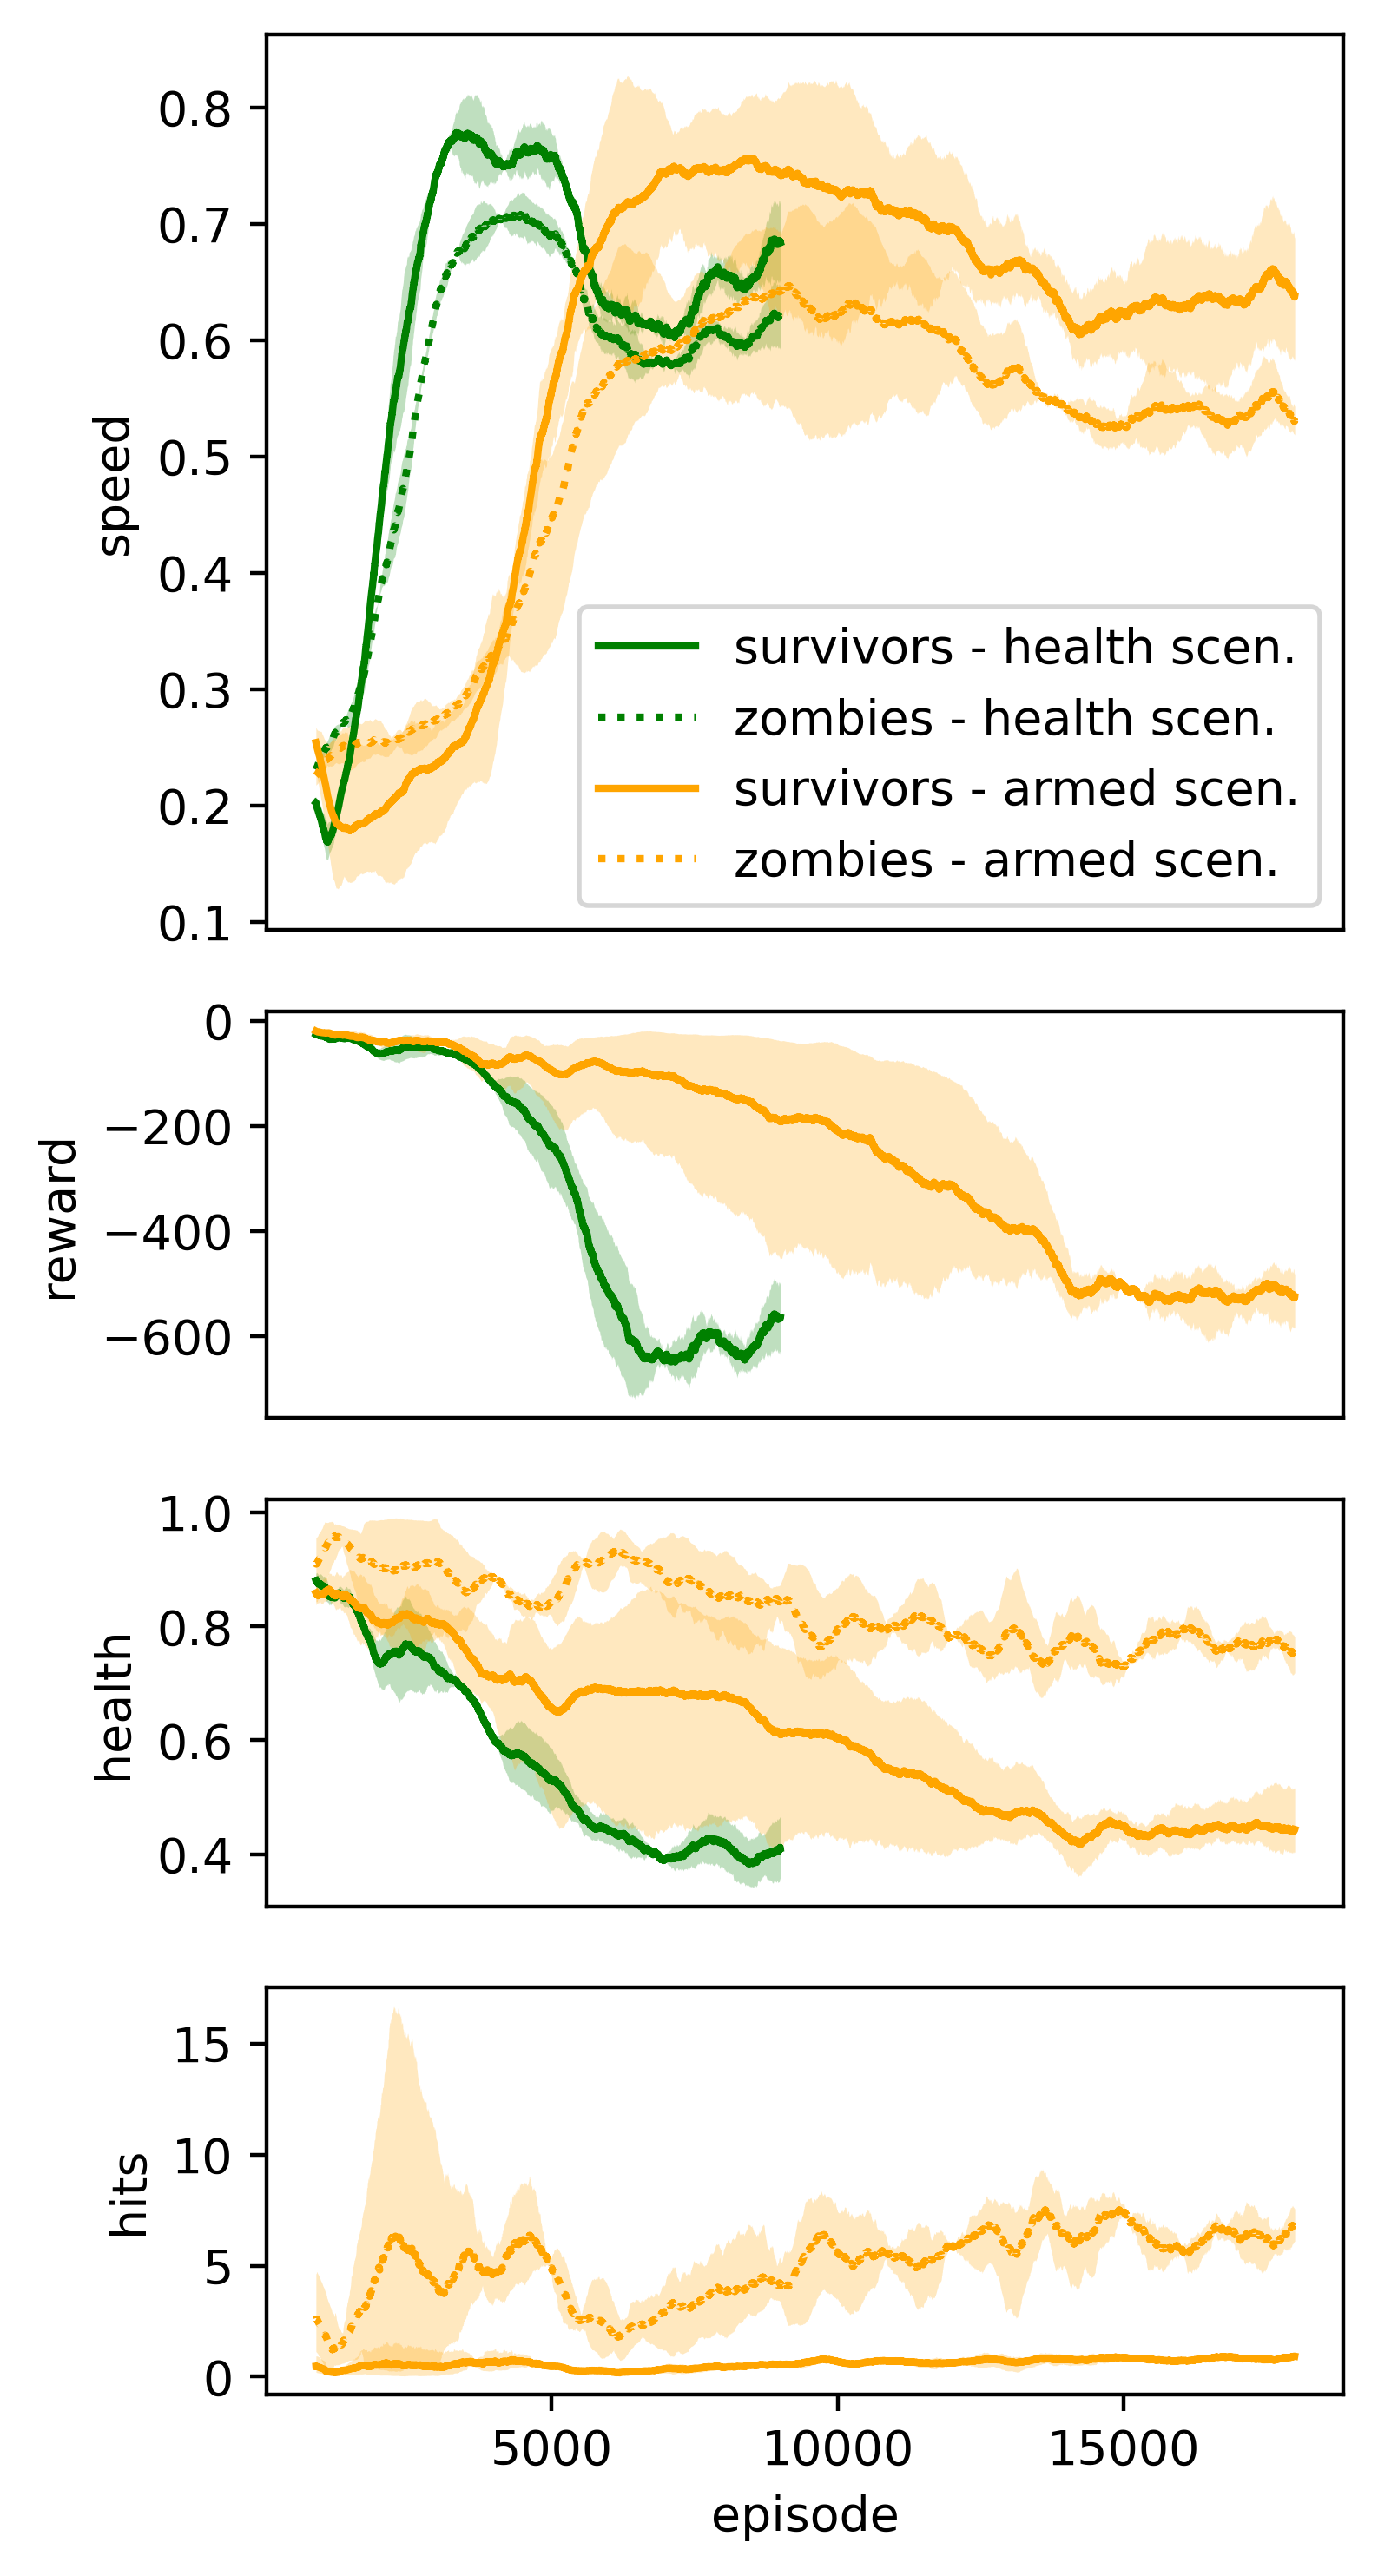
\includegraphics[width=0.5\textwidth]{figures/armed_health_compare.png}
  \caption{
    Comparison between \emph{armed} and \emph{health} scenario policy evolution over 3 training runs.
    Results taken as moving averages over 500 episodes prior to aggregation.
    Plot 1: average speed zombies and survivors per episode.
    Plot 2: survivor episode reward.
    Plot 3: episode-end health of zombies and survivors.
    Plot 4: total hits recieved by zombies and survivors.
  }
  \label{fig:armed_health_compare}
\end{figure}

\begin{figure}
  \centering
  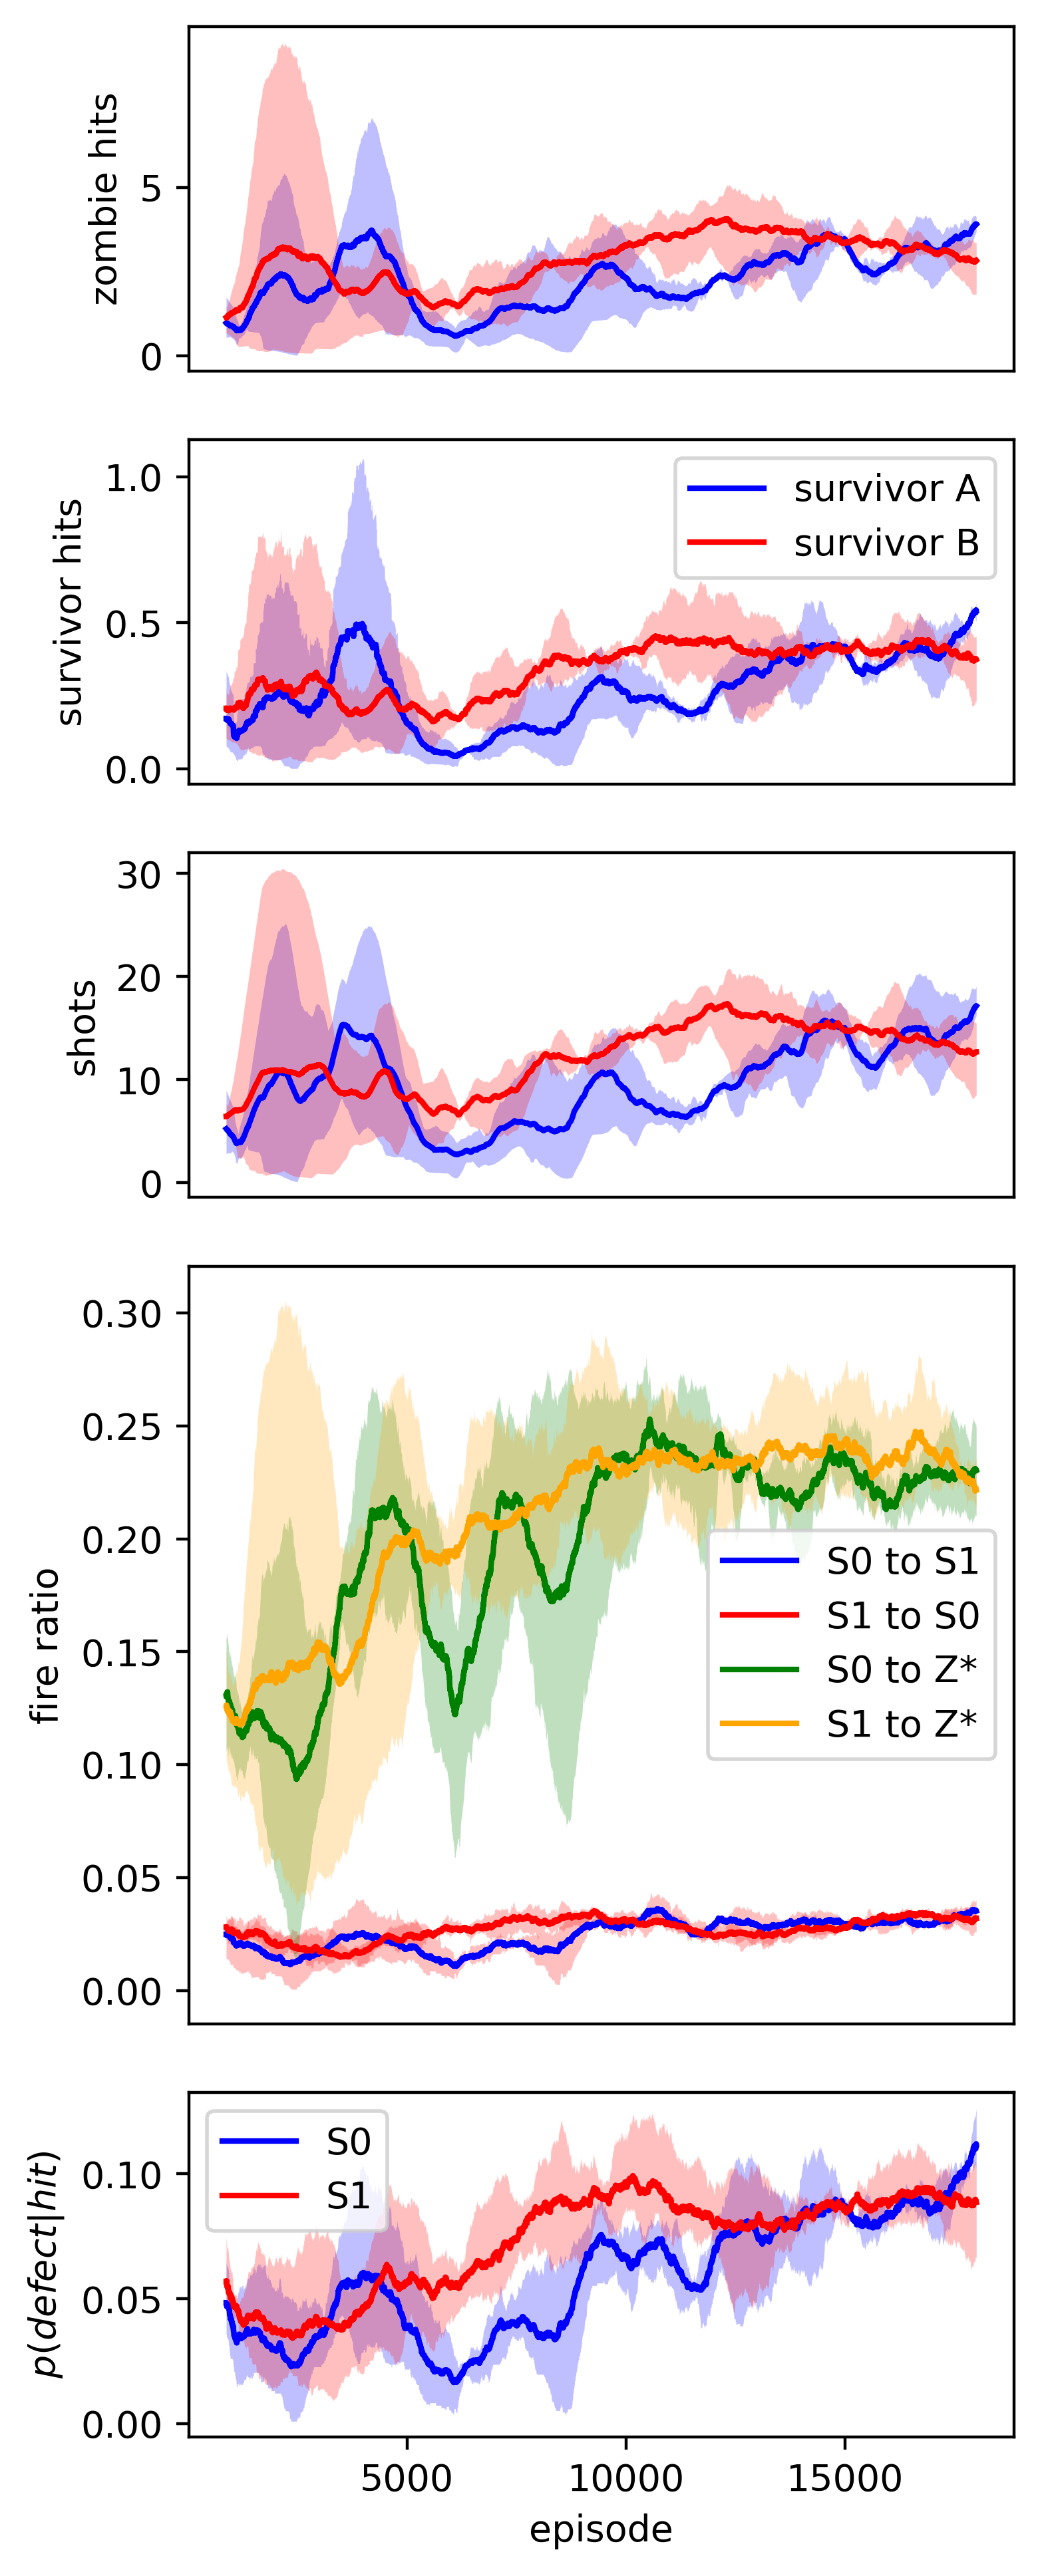
\includegraphics[width=0.5\textwidth]{figures/survivor_skill.png}
  \caption{
    Comparison of hits from different survivors in the \emph{armed} scenario over 3 training runs.
    Results taken as moving averages over 1000 episodes prior to aggregation due to high variance.
    Plot 1: zombie hit counts for each survivor.
    Plot 2: survivor hit counts for each survivor.
    Plot 3: shots fired for each survivor.
    Plot 4: ratio of zombie and survivor hit counts to shots fired for each survivor.
    Plot 5: probability a survivor shot the other survivor, conditional on them having fired and hit something, normaled for team size.
  }
  \label{fig:survivor_skill}
\end{figure}

As expected, the introduction of projectile weapons in the \emph{armed} scenario increased survivor health and rewards on average (Figure \ref{fig:armed_health_compare}, plots 2-3),
shifting the balance of power back toward the survivors.
Relative to the \emph{health} scenario, survivors took longer to learn to increase average speed (Figure \ref{fig:armed_health_compare}, plot 1).
This can be explained by the introduction of a mechanicm for reducing zombie health (the guns), leading to lower average maximum speeds for zombies,
decreasing the urgency with which survivors must learn to move faster.

Interestingly, the initial period (episodes 2000-4000) that survivors in the \emph{health} scenario used to learn increased speed
is used by survivors in the \emph{armed} scenario to learn increased fire rate.

\paragraph{Specialization}
During this phase we found one survivor was often faster than the other at learning to hit targets (Figure \ref{fig:survivor_skill}, plot 1).
The difference in rate of fire in survivors persists over a period and may be indicative of role specialization,
where one survivor learns a benefit from shooting while the other finds more benefit in learning evasion.

\paragraph{More practice required}
After the initial phase, average survivor speed increased to a similar level to that observed in the \emph{health} scenario.
Survivors were able to hold back the zombies initially, but the zombie's power-in-numbers eventually overcame the survivor's advantage.
Examining the zombie hit count compared to the survivor shots fired (Figure \ref{fig:survivor_skill}, plots 1, 3)
indicates that survivors did not become sharpshooters within the number of simulated episodes.
We think this could be improved slightly by simplifying the firing action, or by increasing the incentive (indirectly) to learn accuracy with more powerful guns and a longer reload time.
Or potentially using transfer learning from a `firing range' scenario.

\paragraph{Social dilemmas}
We observed the emergence of another competitive strategy among survivors.
In some episodes we noticed a survivor would occasionally shoot another survivor.
The slowdown caused to the target by the shot would sometimes cause them to become overrun with zombies,
leaving the shooter free of zombie aggravation.

To establish whether this was a strategy and not just chance
we modelled the conditional probability of defection (shooting another survivor) as a Bernoulli trial
in which the survivor, having fired and hit something, has either hit the other survivor or a zombie.

\begin{equation}
  p_i(defect|hit, i\in S) = \frac{
    \sum\limits_{j\neq i, j\in S} h_{i,j}
  }{
    \sum\limits_{j\neq i, j\in S} h_{i,j}
    +
    \sum\limits_{j\in Z} h_{i,j}
  }
\end{equation}

where $h_{i,j}$ is the number of times agent $i$ shot agent $j$ in an episode, $S$ is the set of survivors and $Z$ the set of zombies.

We found that if we accept the model then survivors are learning that if they can hit an agent, a survivor is higher value target than a zombie (Figure \ref{fig:survivor_skill}, plot 5).
We were unable to train the model for more than 20,000 episodes (due to time constraints) to determine if defection emerges as a dominant strategy over time.

\section{Discussion}
\label{sec:discussion}

In attempting to design scenarios to model a `real-life' zombie-survival situation we witnessed the emergence of surprising behaviors.
In each case, our surprise was a result of the environment's dynamics (as implemented) not matching our expectations.

In the \emph{baseline} scenario, we didn't expect target-fixation because our personal state-space representation was already abstracting the agents into two teams.
When we aligned the state-space using our personal abstractions in the \emph{anonymous} scenario the behavior was corrected, but we encountered further surprises.
We did not expect the wall-bouncing strategy because our personal expectation was that running into a wall when chased by zombies is counterproductive.

Our explanation for this assumption was to do with health, which we weren't modelling.
Once we corrected this in the \emph{health} scenario the strategy became less common and we observed the behavior we expected.

In the \emph{armed} scenario we weren't certain how agents would respond.
Survivors were less effective than expected within the training time at using weapons, likely because we underestimated the complexities of a task achievable by humans (in popular depictions of zombie-survivor scenarios, survivors are adept at shooting).
The social dilemma presented warrants further study;
a more thorough empirical game theoretic analysis such as performed in \citealp{10.5555/3091125.3091194} would be an interesting exercise.

We found it an interesting challenge to attempt to produce desired behavior in a multi-agent setting.
Above all, we learned that agents will seek to maximize their reward functions, rather than do what you expect them to do.

\begin{figure}
  \centering
  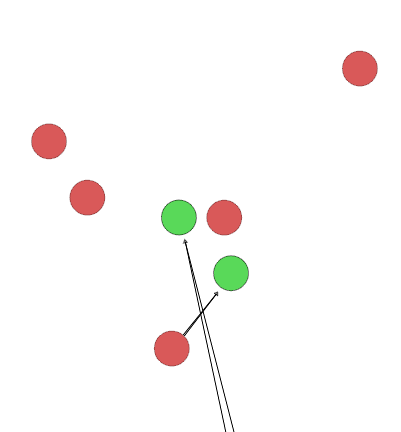
\includegraphics[width=0.5\textwidth]{figures/screencapture.png}
  \caption{
    The \emph{armed} environment.
    Survivors in green, zombies in red.
    Both survivors are firing weapons.
  }
  \label{fig:baseline_reward}
\end{figure}

\bibliography{paper}
\bibliographystyle{acl_natbib}

\end{document}
